\chapter{Strictly Constant Trajectories}

\section{Strictly Constant Trajectories}
\begin{dfn}
	A strictly constant trajectory $x(t) \in \mathbb{R}^n$ for $\dot{x}_i = \sum_{j=1}^n a_{ij}x_j$ satisfies $\dot{x}_i = 0$ and $x_i \neq 0$ for all $i$
\end{dfn}
\begin{thm}
	Suppose $A$ is an irreducible matrix of order $> 2$ and $SD(A)$ has no $k$-cycle, $k > 2$. Then there exist $\tilde{A} \in Q(A)$ and a strictly constant trajectory satisfying $\dot{x}$ = $\tilde{A}x = 0$ if and only if each end node of $SD(A)$ is distinguished and $SD(A)$ is not $\lambda$-consistent.
\end{thm}

\begin{proof}
	Suppose $x$ is a strictly constant trajectory. Since each component of $x$ must be non-zero, it follows that each end node of $SD(A)$ must correspond to a distinguished node in $A$. Furthermore, if $SD(A)$ were $\lambda$-consistent, the existence of non-zero constants $\lambda_1, \lambda_2, \ldots, \lambda_n$ such that $\lambda_i\tilde{a}_{ij} = -\lambda_j\tilde{a}_{ji}$ for all $i \neq j$ in ${1, \ldots, n}$. The subsystem
	
	\begin{equation}
		\dot{x}_i = \sum_{j=1}^n \tilde{a}_{ij}x_j \qquad (i = 1, \ldots, n)
	\end{equation}
	
	then admits the positive definite Lyapunov function
	
	\begin{equation}
		\Lambda(x) = \sum_{i=1}^k \lambda_ix_i^2,
	\end{equation}
	
	whose derivative
	
	
	$$\dot{\Lambda}(x) = \sum_{i=1}^n 2\lambda_ix_i\dot{x}_i = 2 \sum_{i=1}^n \sum_{j=1}^n \lambda_ix_i\tilde{a}_{ij}x_j = 2 \sum_{i=1}^n \lambda_i\tilde{a}_{ii}x_i^2 $$

	Hence, the derivative of $\Lambda$ = $\sum_{i=1}^n \lambda_i x_i^2$ along the constant trajectory $x$ would yield $ 0 = \dot{\Lambda} = 2\sum_{i=1}^n \lambda_i \tilde{a_{ii}}x_i^2 > 0$,  which contradicts the fact that $x$ is a strictly constant trajectory.
	
	For the \textbf{converse}, let us assume $SD(A)$ is itself a proper subchain. Labeling the nodes in the obvious way, $\tilde{A}$ is a tridiagonal matrix; we fix all entries except $\tilde{a}_{nn}$ ($\neq 0$). Considering the disjoint cycles of $A$ and setting $\alpha_i =\tilde{a}_{ii+1}\tilde{a}_{i+1i}$ for $i = 1,2,\ldots,n-1$ gives
	
	\begin{equation}
		\det A = \begin{cases}
			(-1)^{(n)/2}[-\tilde{a}_{11}\alpha_2\alpha_4\cdots\alpha_{n-2}\tilde{a}_{nn} + \alpha_1\alpha_3\cdots\alpha_{n-1}] & \text{if $n$ is even,} \\
			(-1)^{(n-1)/2}[\tilde{a}_{11} \alpha_2\alpha_4\cdots\alpha_{n-1} + \alpha_1\alpha_3\cdots\alpha_{n-2}\tilde{a}_{nn}] & \text{if $n$ is odd.}
		\end{cases}
	\end{equation}
	
	
	The sign of $\tilde{a_{nn}}$ is either $+$ or $-$, and it is either possible to adjust the magnitude of $\tilde{a_{nn}}$ so $\det \tilde{A} = 0$ or not, depending only on that sign. If $SD(A)$ were $\lambda$-consistent, it would be impossible to have a constant trajectory with $\det \tilde{A} = 0$ because of the above argument. Since we are assuming that $SD(A)$ is not $\lambda$-consistent, $\tilde{a_{nn}}$ must be of the other sign, so for some choice of $|\tilde{a_{nn}}|$, $\det A = 0$.
	
	Now let $x$ be a nontrivial solution of $\tilde{A}x = 0$ with $\tilde{A}$ as above. The equations $\sum_{j=1}^n \tilde{a_{ij}}x_j = 0$ with $\tilde{a_{11}} \neq 0$ and $x_1 = 0$ implies $x_2 = 0$, $x_3 = 0$, and so on through the chain; therefore $x_1 \neq 0$. But $x_1 \neq 0$ implies, by the same argument, that each component of $x$ is nonzero. So ,this ensures the existence of a non-trivial solution $x$ to the equation $\tilde{A}x = 0$, where all components of $x$ are non-zero.and so $x$ is a strictly constant trajectory. (Note that if an end node is not distinguished, then the argument fails, as some component of $x$ is zero).
	
	Next suppose that $SD(A)$ may be partitioned into a proper subchain which is not $\lambda$-consistent and a second subchain with exactly one distinguished node, the end node (not the node of attachment); \textbf{see Figure 2.1} for an example.We can construct $\tilde{A}$ and $x$ as before for the proper subchain, and then extend the solution $x$ to the second subchain by recursively specifying the remaining components. The key idea is to use the equations at the attachment node to ensure that the full vector $x$ satisfies $\tilde{A}x = 0$ with all components non-zero.
	
	Starting at the node of attachment $q$, let the nodes of the second subchain be labeled $q,q+1,\ldots, q+m$, with $q+m$ the end node and $a_{q+m,q+m} \neq 0$. Let $\tilde{A}$, $x$ be specified as above for the proper subchain, and let other $\tilde{A}$ entries be arbitrary in magnitude except $\tilde{a}_{q+1,q}$. Tentatively set $x_{q+m} = 1$. Then $x_{q+m-1}$ can be used to specify $x_{q+m-2}$, which in turn can be used to specify $x_{q+m-3}$, and so on down the chain. Finally $x_{q+1}$ is specified.
	
	If there is a sign conflict in the equation at node $q+1$, start over with $x_{q+1} = -1$. Then specify $\tilde{a}_{q+1,q}$. At node $q$ we must modify $\lambda$-values so that $\tilde{a}_{q\alpha}x_{\alpha}+ \tilde{a}_{q\beta}x_{\beta} +\tilde{a}_{qq+1}x_{q+1}  = 0$, where nodes $\alpha,\beta$ are neighbors of node $q$ in the proper subchain. The first two summands are already of opposite signs, so adjustment of the magnitudes of $\tilde{a}_{q\alpha}$ and $\tilde{a}_{q\beta}$ can clearly be carried out so $\tilde{A}x = 0$, all $x_i \neq 0$, $i=q,\ldots,q+m$. The case in which the node of attachment $q$ is also distinguished follows in a similar way, with the additional term $\tilde{a}_{qq}x_q$ in the equation at node $q$.
	
	A simple extension of the above sequence shows that any number of subchains with distinguished end nodes can be accommodated. Lastly, additional nodes can acquire (small magnitude) 1-cycles by local adjustment of $\tilde{A}$ values, since each node clearly has inputs of opposite signs.
\end{proof}
	\begin{figure}[h]
		\centering
		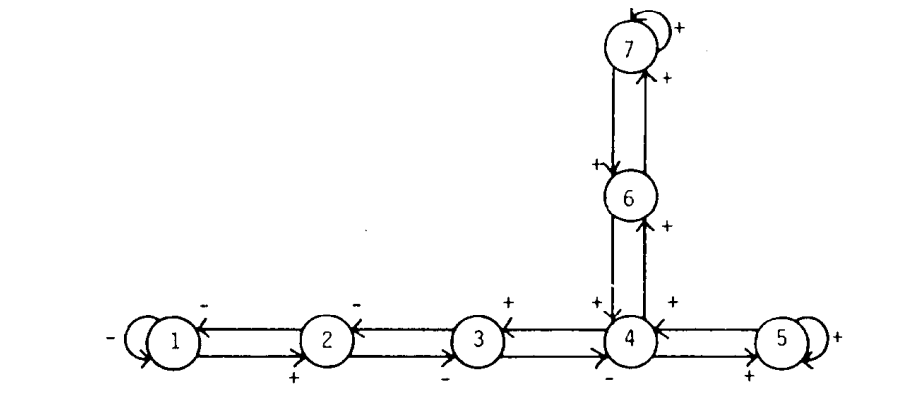
\includegraphics[height= 6.5cm]{Figure1.png}
		\caption{An example to illustrate method of proof of Theorem 1. Nodes $\{1,2,3,4,5\}$ are in proper subchain and nodes 4,6,7 are in a second subchain with the end end distinguished}
	\end{figure}

	\begin{example}
		In our example, suppose that $SD(A)$ can be divided into a proper subchain that is not $\lambda$-consistent and a second subchain with exactly one distinguished node, denoted as node 7, which serves as the end node (but not the attachment node). Let $\tilde{A}$ and $x$ be specified as described for the proper subchain, which includes nodes $\{1,2,3,4,5\}$, and let the other entries of $\tilde{A}$ be arbitrary in magnitude except for $\tilde{a_{q+1q}}=\tilde{a_{64}}$.
		
		Based on the given signed digraph $SD(A)$, consider the matrix given by:
		\begin{center}
			$\tilde{A} = \begin{bmatrix}
				1 & 2 & 0 & 0 & 0 & 0 & 0\\
				1 & 0 & -1 & 0 & 0 & 0 & 0\\
				0 & -2 & 0 & -1 & 0 & 0 & 0 \\
				0 & 0 & 1 & 0 &2 & -1 & 0\\
				0 & 0 & 0 & 1 & 2 & 0 & 0\\
				0 & 0 & 0 &\tilde{a_{64}}&0 & 0 & 1\\
				0 & 0 & 0 & 0 &0 & 1 & 1
			\end{bmatrix}$
			and $x= \begin{bmatrix}
				-2\\
				1 \\
				-2\\
				-2\\
				1\\
				x_6\\
				x_7\\
			\end{bmatrix}$
		\end{center}
		
		Solving by the algorithm outlined in the theorem's proof:
		\begin{enumerate}
			\item Set $x_7=1$ and solve the equation $\tilde{A}x=0$ at node 7, resulting in $x_6=-1$.
			\item Specify the value of $\tilde{a_{64}}$ by solving the equation at node 6, yielding $\tilde{a_{64}} = 1/2$.
			\item Modify the values of $\tilde{A}$ at the attachment node, i.e., node 4, to satisfy the equation at node 4 given by:
			\[\tilde{a_{43}}x_{3} + \tilde{a_{45}}x_{5} + \tilde{a_{46}}x_{6} = 0\]
			Set $\tilde{a_{43}} = 3/2$, resulting in the final $\tilde{A}$ and $x$:
		\end{enumerate}
		
		\begin{center}
			$\tilde{A} = \begin{bmatrix}
				-1 & 2 & 0 & 0 & 0 & 0 & 0\\
				1 & 0 & -1 & 0 & 0 & 0 & 0\\
				0 & -2 & 0 & -1 & 0 & 0 & 0 \\
				0 & 0 & 1 & 0 &2 & -1 & 0\\
				0 & 0 & 0 & 1 & 2 & 0 & 0\\
				0 & 0 & 0 & 1/2&0 & 0 & 1\\
				0 & 0 & 0 & 0 &0 & 1 & 1
			\end{bmatrix}$
			and $x= \begin{bmatrix}
				-2\\
				1 \\
				-2\\
				-2\\
				1\\
				-1\\
				1\\
			\end{bmatrix}$
		\end{center}
		
	\end{example}